\documentclass[a4paper,12pt]{article} % тип документа

% Поля страниц
\usepackage[left=2.5cm,right=2.5cm,
    top=2cm,bottom=2cm,bindingoffset=0cm]{geometry}
 

\DeclareUnicodeCharacter{2206}{$\Delta$}
\DeclareUnicodeCharacter{03C1}{$\rho$}

%Отступ после заголовка    
\usepackage{indentfirst}


% Рисунки
\usepackage{floatrow,graphicx,calc}
\usepackage{wrapfig}

% Создаёем новый разделитель
\DeclareFloatSeparators{mysep}{\hspace{1cm}}

% Ссылки?
\usepackage[unicode, pdftex]{hyperref} % подключаем hyperref
\usepackage{hyperref}
\usepackage[rgb]{xcolor}
\hypersetup{				% Гиперссылки
    colorlinks=true,       	% false: ссылки в рамках
	urlcolor=blue          % на URL
}


%  Русский язык
\usepackage[T2A]{fontenc}			% кодировка
\usepackage[utf8]{inputenc}			% кодировка исходного текста
\usepackage[english,russian]{babel}	% локализация и переносы


% Математика
\usepackage{amsmath,amsfonts,amssymb,amsthm,mathtools}


% Что-то 
\usepackage{wasysym}

\begin {document}

\begin{titlepage}
\newcommand{\HRule}{\rule{\linewidth}{0.3 mm}} % Defines a Hnew command for the horizontal lines, change thickness here

\center % Center everything on the page
 
%----------------------------------------------------------------------------------------
%	HEADING SECTIONS
%----------------------------------------------------------------------------------------

\textsc{\Large Московский физико-технический институт }\\[1.5cm] % Name of your university/college
\textsc{\Large Факультет аэрокосмических технологий}\\[0.5cm] % Major heading such as course name
\textsc{\large Лабораторная работа 2.3.1}\\[0.5cm] % Minor heading such as course title

%----------------------------------------------------------------------------------------
%	TITLE SECTION
%----------------------------------------------------------------------------------------

\HRule \\[0.4cm]
{ \huge \bfseries Получение и измерение вакуума }\\[0.4cm] % Title of your document
\HRule \\[1.5cm]
 
%----------------------------------------------------------------------------------------
%	AUTHOR SECTION
%----------------------------------------------------------------------------------------

\begin{minipage}{0.4\textwidth}
\begin{flushleft} \large
\emph{Автор:}\\ Артем \textsc{Овчинников} % Your name
\end{flushleft}
\end{minipage}
\begin{minipage}{0.4\textwidth}
\begin{flushright} \large
\emph{Преподаватель:} \\
Арина Владимировна \textsc{Радивон} % Supervisor's Name
\end{flushright}
\end{minipage}\\[4cm]
%	DATE SECTION
%----------------------------------------------------------------------------------------

{\large \today}\\[2cm] % Date, change the \today to a set date if you want to be precise

%----------------------------------------------------------------------------------------
%	LOGO SECTION
%----------------------------------------------------------------------------------------

 
%----------------------------------------------------------------------------------------

\vfill % Fill the rest of the page with whitespace

\end{titlepage}
\tableofcontents
\newpage
\section{Аннотация}
Цель работы: 1) измерение объемов орвакуумной и высоковаку
умной частей установки; 2) определение скорости откачки системы в
стационарном режиме, а также по ухудшению и по улучшению вакуума. \\
В работе используются: вакуумная установка с манометрами: масляным, термопарным и ионизационным. 
\section{Теоретические сведения}

	Производительность насоса определяется скоростью откачки $W$ (л/с): $W$ — это объем газа, удаляемого из сосуда при данном давлении за единицу времени. Скорость откачки форвакуумного насоса равна емкости воздухозаборной камеры, умноженной на число оборотов в секунду.
Рассмотрим обычную схему откачки. Разделим вакуумную систему на две части: «откачиваемый объем» (в состав которого включим используемые для работы части установки) и «насос», к которому, кроме самого насоса, отнесем трубопроводы и краны, через которые
производится откачка нашего объема. Обозначим через $Q_d$ количество газа, десорбирующегося с поверхности откачиваемого объема в единицу времени, через $Q_i$ — количество газа, проникающего в единицу времени в этот объем извне — через течи. Будем считать, что насос обладает скоростью откачки $W$ и в то же время сам является источником газа; пусть $Q_n$ — поток газа, поступающего из насоса назад в откачиваемую систему. Будем измерять количество газа $Q_d$, $Q_i$ и $Q_n$ в единицах $PV$ (легко видеть, что это произведение с точностью до множителя $RT/ \mu$ равно массе газа). Основное уравнение, описывающее процесс откачки, имеет вид

\begin{equation}
\label{otkachka}
	-VdP=(PW-Q_d-Q_n-Q_i)dt.
\end{equation}

Левая часть этого уравнения равна убыли газа в откачиваемом объеме $V$ , а правая определяет количество газа, уносимого насосом, и количество прибывающего вследствие перечисленных выше причин
за время $dt$. При достижении предельного вакуума (давление $P_{pr}$)

\begin{equation}
\label{predel_1}
	\frac{dP}{dt}=0,
\end{equation}

\begin{equation}
\label{predel_2}
	W=\frac{\sum Q_i}{P_{pr}}.
\end{equation}

Обычно $Q_i$ постоянно, a $Q_n$ и $Q_d$ слабо зависят от времени, поэтому в наших условиях все эти члены можно считать постоянными. Считая также постоянной скорость откачки $W$ , уравнение~(\ref{otkachka}) можно проинтегрировать и, используя~(\ref{predel_1}), получить
\begin{equation}
\label{davlenie}
	P = P_o \exp{(-\frac{W}{V} t)} + P_{pr}.
\end{equation}

	Характер течения газа существенно зависит от соотношения между размерами системы и длиной свободного пробега молекул. При атмосферном давлении и даже при понижении давления до форвакуумного длина свободного пробега меньше диаметра трубок и течение откачиваемого газа определяется его вязкостью, т. е. взаимодействием его молекул. При переходе к высокому вакууму картина меняется. Столкновения молекул между собой начинают играть меньшую роль, чем соударения со стенками. Течение газа в трубе напоминает в этих условиях диффузию газа из области больших концентраций в области, где концентрация ниже, причем роль длины свободного пробега играет ширина трубы.
Для количества газa, протекающего через трубу в условиях высокого вакуума или, как говорят, в кнудсеновском режиме, справедлива формула

\begin{equation}
\label{formula}
	\frac{d(PV)}{dt}=\frac{4}{3}r^3 \sqrt{\frac{2\pi RT}{\mu}} \frac{P_2-P_1}{L}.
\end{equation}
Применим эту формулу к случаю, когда труба соединяет установку с насосом.
Пренебрежем давлением $P_1$ у конца, обращенного к насосу. Будем измерять количество газа, покидающего установку при давлении $P = P_2$. Пропускная способность трубы

\begin{equation}
	C_{tr}=(\frac{dV}{dt})_{tr}=\frac{4}{3}\frac{r^3}{L}\sqrt{\frac{2\pi RT}{\mu}}.
\end{equation}

	Мы видим, что пропускная способность зависит от радиуса трубы в третьей степени и обратно пропорциональна ее длине. В вакуумных установках следует поэтому применять широкие короткие  трубы.
	
	При расчете вакуумных систем нужно принимать во внимание также пропускную способность отверстий, например, в кранах. Для диффузионного насоса можно считать, что каждая молекула воздуха, попавшая в кольцевой зазор между соплом и стенками насоса, увлекается струей пара и не возвращается обратно в откачиваемый объем. Скорость откачки такого насоса можно считать равной пропускной способности отверстия с площадью, равной площади кольцевого зазора, т. е. насос качает как кольцевой зазор, с одной стороны которого расположен откачиваемый объем, а с другой -- пустота.


\section{Методика измерений}

При работе с насосом следует помнить, что после остановки насоса
в него обязательно нужно впускать воздух. Если этого не делать, то
атмосерное давление может выдавить масло из насоса в патрубки и в
вакуумную систему. Соединять насос с атмосерой следует при помощи
кранов К1 или К2.
После включения насоса его присоединяют к установке не сразу, а
через некоторое время, когда насос откачает собственный объјм и про-
странство, расположенное до крана К2. Об этом можно судить по звуку
насоса. Вначале насос сильно шумит, затем его звук делается мягким,
и, наконец, в насосе возникает сухой стук, это происходит, когда до-
стигается хорошее разрежение.

\section{Используемое оборудование}

Экспериментальная установка. Установка изготовлена из стекла и
состоит из орвакуумного баллона (ФБ), высоковакуумного диузи-
онного насоса (ВН), высоковакуумного баллона (ВБ), масляного (М) и
ионизационного (И) манометров, термопарных манометров (М1 и M2),
орвакуумного насоса (ФН) и соединительных кранов К1, К2, ..., К6
(рис. 1). Кроме того, в состав установки входят: вариатор (автотранс-
орматор с регулируемым выходным напряжением), или реостат, и ам-
перметр для регулирования тока нагревателя диузионного насоса. \\

Форвакуумный насос. Устройство и принцип действия ротационного
пластинчатого орвакуумного насоса схематически показаны на рис. 2.
В цилиндрической полости массивного корпуса размещен эксцен-
трично ротор так, что он постоянно соприкасается своей верхней частью
с корпусом. В диаметральный разрез ротора вставлены две пластины,
раздвигаемые пружиной и плотно прижимаемые к поверхности полости.
Они разделяют объјм между ротором и корпусом на две части. \\

Диффузионный насос. Откачивающее действие диузионного на-
соса основано на диузии (внедрении) молекул разреженного воздуха
в струю паров масла. Попавшие в струю молекулы газа увлекаются ею
и уже не возвращаются назад. На прежнем их месте образуется пустота,
которая немедленно заполняется следующими порциями газа, увеличи-
вая степень разрежения газа в окрестности струи и оказывая таким
образом сильное откачивающее воздействие на весь газ в откачиваемом
объјме. Скорость откачки диузионных насосов в сотни и тысячи раз
превосходит скорость откачки орвакуумного насоса.  \\

\section{Результаты измерений и обработка данных}

\floatsetup[table]{capposition=top}	
\begin{table}[H]
	\caption{Результаты измерений}
	\label{table:main}
\begin{tabular}{lllllll}
t, s & P, 10\textasciicircum{}(-4)mmHg &  &  &  &  &  \\
0    & 1.8                              &  &  &  &  &  \\
5    & 1.8                              &  &  &  &  &  \\
10   & 1.8                              &  &  &  &  &  \\
15   & 2.2                              &  &  &  &  &  \\
20   & 2.9                              &  &  &  &  &  \\
25   & 3.7                              &  &  &  &  &  \\
30   & 4.5                              &  &  &  &  &  \\
35   & 5.2                              &  &  &  &  &  \\
40   & 5.9                              &  &  &  &  &  \\
45   & 6.5                              &  &  &  &  &  \\
50   & 7.3                              &  &  &  &  &  \\
55   & 7.9                              &  &  &  &  &  \\
60   & 5.8                              &  &  &  &  &  \\
65   & 2.4                              &  &  &  &  &  \\
70   & 1.9                              &  &  &  &  &  \\
75   & 1.8                              &  &  &  &  & 
\end{tabular}
\end{table}

\thisfloatsetup{floatrowsep=mysep}	
\begin{figure}[H]
\begin{floatrow}
 \ffigbox[\FBwidth]{\caption{{{График зависимости $ln (\frac{P-P_{lim}}{P_0})(t)$}}}\label{fig:Graph_5}}%
         {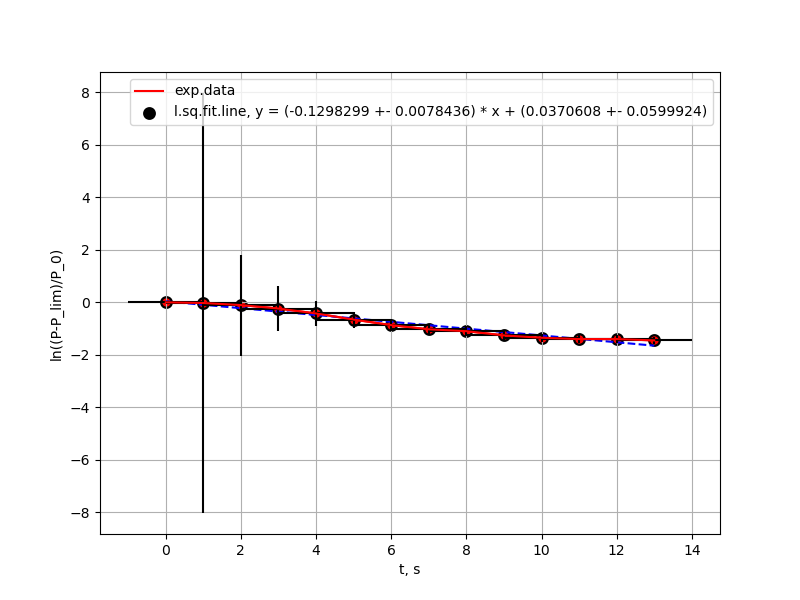
\includegraphics[scale=0.75]{physlabwork_15week_dlogPdt.png}}     
\end{floatrow}
\end{figure}

\begin{equation*}
    \frac{W}{V} = 0.13 \frac{1}{s}
\end{equation*}

\begin{equation*}
    W = 0.28 \frac{L}{s}
\end{equation*}

\section{Обсуждение результатов}

\section{Выводы}

\end{document}
